\documentclass[xcolor=table]{beamer}
%\documentclass[handouts]{beamer}
%\setbeameroption{show notes}
\setbeameroption{hide notes}
%\setbeameroption{show only notes}


%[xetex,mathserif,serif]
\usepackage{multicol}
%\usepackage{animate}
\usepackage{verbatim}
\makeatletter
\newcommand{\verbatimfont}[1]{\renewcommand{\verbatim@font}{\ttfamily#1}}
\makeatother
\usepackage{hyperref}
\usepackage{tikz}

\graphicspath{{images/}}

%KTH official colors https://intra.kth.se/polopoly_fs/1.486828!/image/fargreferens_png.png
\definecolor{kthBlue}{RGB}{25,84,166} %Bla
\definecolor{kthLightBlue}{RGB}{36,160,216} %Ljusbla

\definecolor{kthRed}{RGB}{157,16,45} %Rod
\definecolor{kthLigthRed}{RGB}{228,54,62} %Lujsrod

\definecolor{kthGrey}{RGB}{101,101,108} %Morkgra
\definecolor{kthLightGrey}{RGB}{227,229,227} %Ljusgra
\definecolor{kthMediumGrey}{RGB}{189,188,188} %Mellangra

\definecolor{kthGreen}{RGB}{98,146,46} %Gorn
\definecolor{kthLightGreen}{RGB}{176,201,43} %Ljusgron


\usetheme{AnnArbor}

% \setbeamercolor{background canvas}{bg=white}
\setbeamercolor*{structure}{fg=kthLightBlue,bg=kthBlue}
\setbeamercolor*{palette primary}{use=structure,fg=white,bg=kthBlue} 
\setbeamercolor*{palette secondary}{use=structure,fg=black,bg=kthLightGrey}
\setbeamercolor*{palette tertiary}{use=structure,fg=black,bg=kthLightBlue}
%\setbeamercolor*{palette quaternary}{use=structure,fg=black,bg=kthLightGrey}


\setbeamercolor*{frametitle}{fg=kthBlue,bg=kthLightGrey}
\setbeamercolor*{alerted text}{fg=kthRed}
\setbeamercolor*{item projected}{fg=white,bg=kthLightBlue}
%\setbeamercolor{palette sidebar primary}{use=structure,fg=structure.fg,bg=red}
%\setbeamercolor{palette sidebar secondary}{use=structure,fg=structure.fg,bg=green}
%\setbeamercolor{palette sidebar tertiary}{use=normal text,fg=normal text.fg}


\setbeamercolor{block title}{bg=kthMediumGrey}
\setbeamercolor{block body}{bg=normal text.bg!90!black}

\setbeamercolor{block title alerted}{use={normal text,alerted text},fg=alerted text.fg!75!normal text.fg,bg=normal text.bg!75!black}
\setbeamercolor{block body alerted}{bg=normal text.bg!90!black}

\setbeamercolor{block title example}{use={normal text,example text},fg=example text.fg!75!normal text.fg,bg=normal text.bg!75!black}
\setbeamercolor{block body example}{bg=normal text.bg!90!black}

%\setbeamercolor{fine separation line}{}
%\setbeamercolor{normal text}{bg=white,fg=black}
%\setbeamercolor{section in sidebar}{fg=red}
%\setbeamercolor{section in sidebar shaded}{fg=grey}
%\setbeamercolor{separation line}{}
%\setbeamercolor{structure}{bg=black, fg=kthGreen}
%\setbeamercolor{subsection in sidebar}{fg=brown}
%\setbeamercolor{subsection in sidebar shaded}{fg=grey}
\setbeamercolor{title}{fg=white,bg=kthBlue}
%\setbeamercolor{titlelike}{fg=DarkGreen}


%\setbeamercolor{sidebar}{bg=red}
%\setbeamercolor{sidebar}{parent=palette primary}
%\setbeamercolor{palette sidebar primary}{fg=red}%use=normal text,fg=normal text.fg}
%\setbeamercolor{palette sidebar quaternary}{fg=red}
%\setbeamercolor{palette sidebar secondary}{use=structure,fg=structure.fg}
%\setbeamercolor{palette sidebar tertiary}{use=normal text,fg=normal text.fg}



\title{Introduction to PDC environment}
\subtitle{}

\author{Thor Wikfeldt}

\institute[PDC]{
  PDC Center for High Performance Computing\\
  KTH Royal Institute of Technology
  }
  \logo{
   
\includegraphics[width=1cm,keepaspectratio]{logo_kth_transparent}~%
   % \includegraphics[width=1cm,height=1cm,keepaspectratio]{logo_kth+pdc_blue}~%
 
}
\date[PDC Oct 2017]{Introduction to PDC, February 2018}
\subject{Introduction}


\begin{document}
\frame{\titlepage}

\AtBeginSection[]
{
  \begin{frame}
    \frametitle{Outline}
    \tableofcontents[currentsection]
  \end{frame}
}
%\AtBeginSubsection[]
%{
 % \begin{frame}
  %  \frametitle{Table of Contents}
   % \tableofcontents[currentsection,currentsubsection]
 % \end{frame}
%}

%\frame[plain]{
%Large image inclusion 
%\color{kthBlue}{kthBlue}\\
%\color{kthLightBlue}{kthLightBlue}\\
%\color{kthRed}{kthRed}\\
%\color{kthLigthRed}{kthLigthRed}\\
%\color{kthGrey}{kthGrey}\\
%\color{kthLightGrey}{kthLightGrey}\\
%\color{kthGreen}{kthGreen}\\
%\color{kthLightGreen}{kthLightGreen}\\
%\color{kthMediumGrey}{kthMediumGrey}
%}
%\frame[shrink]{
%%\begin{block}{Answered Questions}
%How many primes are there?
%\end{block}
%\begin{block}{Open Questions}
%Is every even number the sum of two primes?
%\end{block}
%}
%\frame[allowframebreaks]{
%The allowframebreaks option will auto-create new frames if there is too much content to be displayed on one.
%}



\newcommand\irregularcircle[2]{% radius, irregularity
  \pgfextra {\pgfmathsetmacro\len{(#1)+rand*(#2)}}
  +(0:\len pt)
  \foreach \a in {10,20,...,350}{
    \pgfextra {\pgfmathsetmacro\len{(#1)+rand*(#2)}}
    -- +(\a:\len pt)
  } -- cycle
}

\section{PDC Overview}
\subsection*{History}

\frame{
\frametitle{History of PDC}

\begin{itemize}
\item In 1988, envisioning that massive parallelism will become important for CS 
and HPC, a group of scientists from KTH School of Computer Science and 
Engineering applied for grant to buy a parallel computer
\item Market was surveyed and it was decided that Thinking Machines
Corporation (TMC) offered the best choice with its Connection Machine system, CM2
\item What was to be called the Center for Parallel Computers was formed and 
inaugurated by Janne Carlsson, the President of KTH, on January 15, 1990
\item In January 1991 PDC applied for an upgrade of the CM2 to a CM200. The
application was successful and the upgrade was installed in December 1991
\end{itemize}
}

\frame{
\frametitle{History of PDC}

\footnotesize 
\begin{table}
\begin{tabular}{r|r|r|r|l|l} \hline 
\textbf{Year} & \textbf{rank} & \textbf{procs.} & \textbf{peak TFlops} & \textbf{vendor} & \textbf{name} \\ \hline
2014 & 32  & 53632 & 1973.7 & Cray & Beskow\footnote{XC40 16-core 2.3GHz} \\ \hline
2011 & 31  & 36384 & 305.63 & Cray & Lindgren\footnote{XE6 12-core 2.1 GHz} \\ \hline
2010 & 76  & 11016 & 92.534 & Cray & Lindgren\footnote{XT6m 12-core 2.1 GHz} \\ \hline
2010 & 89  & 9800  & 86.024 & Dell & Ekman\footnote{PowerEdge SC1435 Dual core Opteron 2.2GHz, Infiniband} \\ \hline
2005 & 65  & 886   & 5.6704 & Dell & Lenngren\footnote{PowerEdge 1850 3.2 GHz, Infiniband} \\ \hline
2003 & 196 & 180   & 0.6480 & HP & Lucidor\footnote{Cluster Platform 6000 rx2600 Itanium2 900 MHz Cluster, Myrinet} \\ \hline
1998 & 60  & 146   & 0.0934 & IBM & Strindberg\footnote{SP P2SC 160 MHz} \\ \hline
1996 & 64  & 96    & 0.0172 & IBM & Strindberg\footnote{SP2/96} \\ \hline
1994 & 341 & 256   & 0.0025 & Thinking Machines & Bellman\footnote{CM-200/8k} \\ \hline
\end{tabular}
\end{table}

}

\subsection*{Member of SNIC}

\frame
{
\frametitle{SNIC}
\framesubtitle{Swedish National Infrastructure for Computing}
\begin{columns}
\column{.4\textwidth}
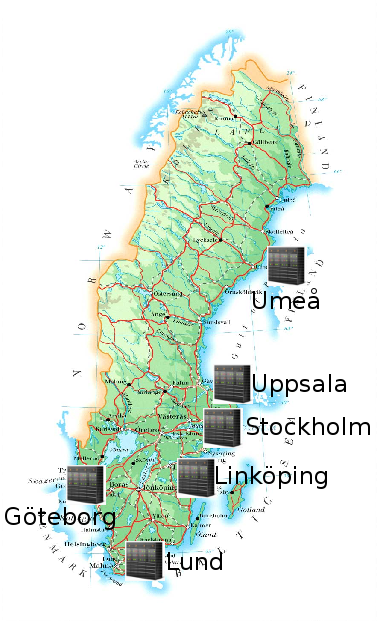
\includegraphics[width=0.8\linewidth]{sweden.png}\\
%\vspace{-55mm}
\column{.6\textwidth}
National \alert{research infrastructure} that provides a \alert{balanced and cost-efficient} set of \alert{resources and user support} for \alert{large scale computation and data storage} to meet the needs of researchers from all scientific disciplines and from all over Sweden (universities, university colleges, research institutes, etc).
\end{columns}
}



\subsection*{EU Access}
\frame{
\frametitle{Access to EU Facilities and Experts}
\begin{columns}
\column{.3\textwidth}

\includegraphics[width=0.9\linewidth]{eudat}\\~\\~\\~\\~\\

\includegraphics[width=0.9\linewidth]{epigram}
%\vspace{-55mm}
\column{.3\textwidth}

\includegraphics[width=0.9\linewidth]{prace}\\~\\

\includegraphics[width=0.9\linewidth]{egi}\\~\\

\includegraphics[width=0.9\linewidth]{einfra}


\column{.3\textwidth}

\includegraphics[width=0.9\linewidth]{cresta}\\

\includegraphics[width=0.9\linewidth]{7}

\end{columns}
}


\subsection*{Industry}
\frame{
\frametitle{PDC and Industry}
Working with industrial researchers and developers on major international projects that push high-performance computing to the next level. 
~\\~\\
Recently established a \alert{business development unit} that provides consultancy and HPC services to industries.
~\\~\\
\begin{columns}
\column{.25\textwidth}

\includegraphics[width=0.7\linewidth]{monotricat}
\column{.25\textwidth}

\includegraphics[width=0.9\linewidth]{ohb}
%\vspace{-55mm}
\column{.25\textwidth}

\includegraphics[width=0.9\linewidth]{pgs}
\column{.25\textwidth}

\includegraphics[width=0.9\linewidth]{scania}
\end{columns}

\begin{columns}
\column{.25\textwidth}

\includegraphics[width=0.7\linewidth]{logo_tyrens}
\column{.25\textwidth}

\includegraphics[width=0.9\linewidth]{fs_dynamics_logo}
\end{columns}

}


\subsection*{Training}
\frame{
\frametitle{Broad Range of Training}
\begin{description}
 \item [Summer School]  Introduction to HPC held every year
 \item [Specific Courses] Programming with GPGPU, Recent Advances in Distributed and Parallel Computing and/or Cloud Computing, Software Development Tools, etc
 \item [PDC User Days] PDC Pub and Open House
\end{description}

\begin{columns}
\column{.3\textwidth}
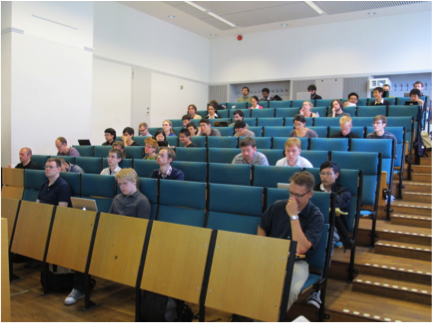
\includegraphics[width=0.9\linewidth]{class3}
\column{.3\textwidth}
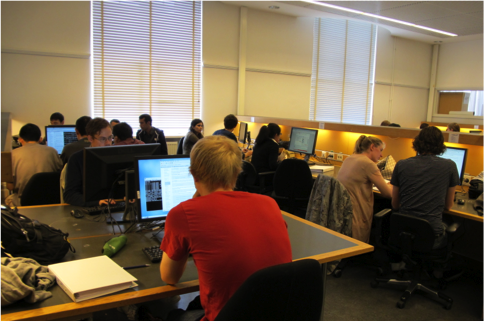
\includegraphics[width=0.9\linewidth]{class2}
\column{.3\textwidth}
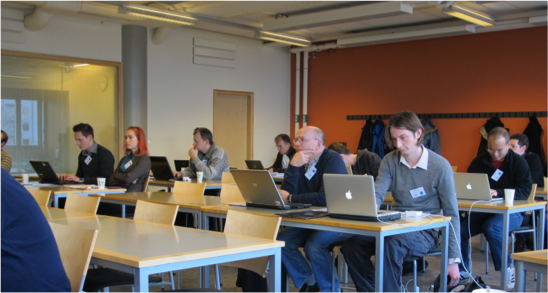
\includegraphics[width=0.9\linewidth]{class1}
\end{columns}
}

\subsection*{Staff}
\frame{
\frametitle{Support and System Staff}
\begin{exampleblock}{First-line support}
  Provide specific assistance to PDC users related to accounts, login, allocations etc.
\end{exampleblock}
\begin{exampleblock}{System staff}
  System managers/administrators ensure that computing and storage resources run smoothly and securely.
\end{exampleblock}
\begin{exampleblock}{Application Experts}
  Hold PhD degrees in various fields and specialize in HPC. Assist researchers in optimizing, scaling and enhancing scientific codes for current and next generation supercomputers.
\end{exampleblock}
}


\frame<presentation:0>[noframenumbering]{
\frametitle{Application Experts}
Hold PhD degrees in different scientific fields and are experts in HPC. Together with researchers, they optimize, scale and enhance scientific codes for the next generation supercomputers.
\footnotesize{
\begin{columns}

\column{.3\textwidth}

\includegraphics[width=0.5\linewidth]{jaime_rosal}\\ \textbf{Jaime Rosal Sandberg} \\ Computational Chemistry
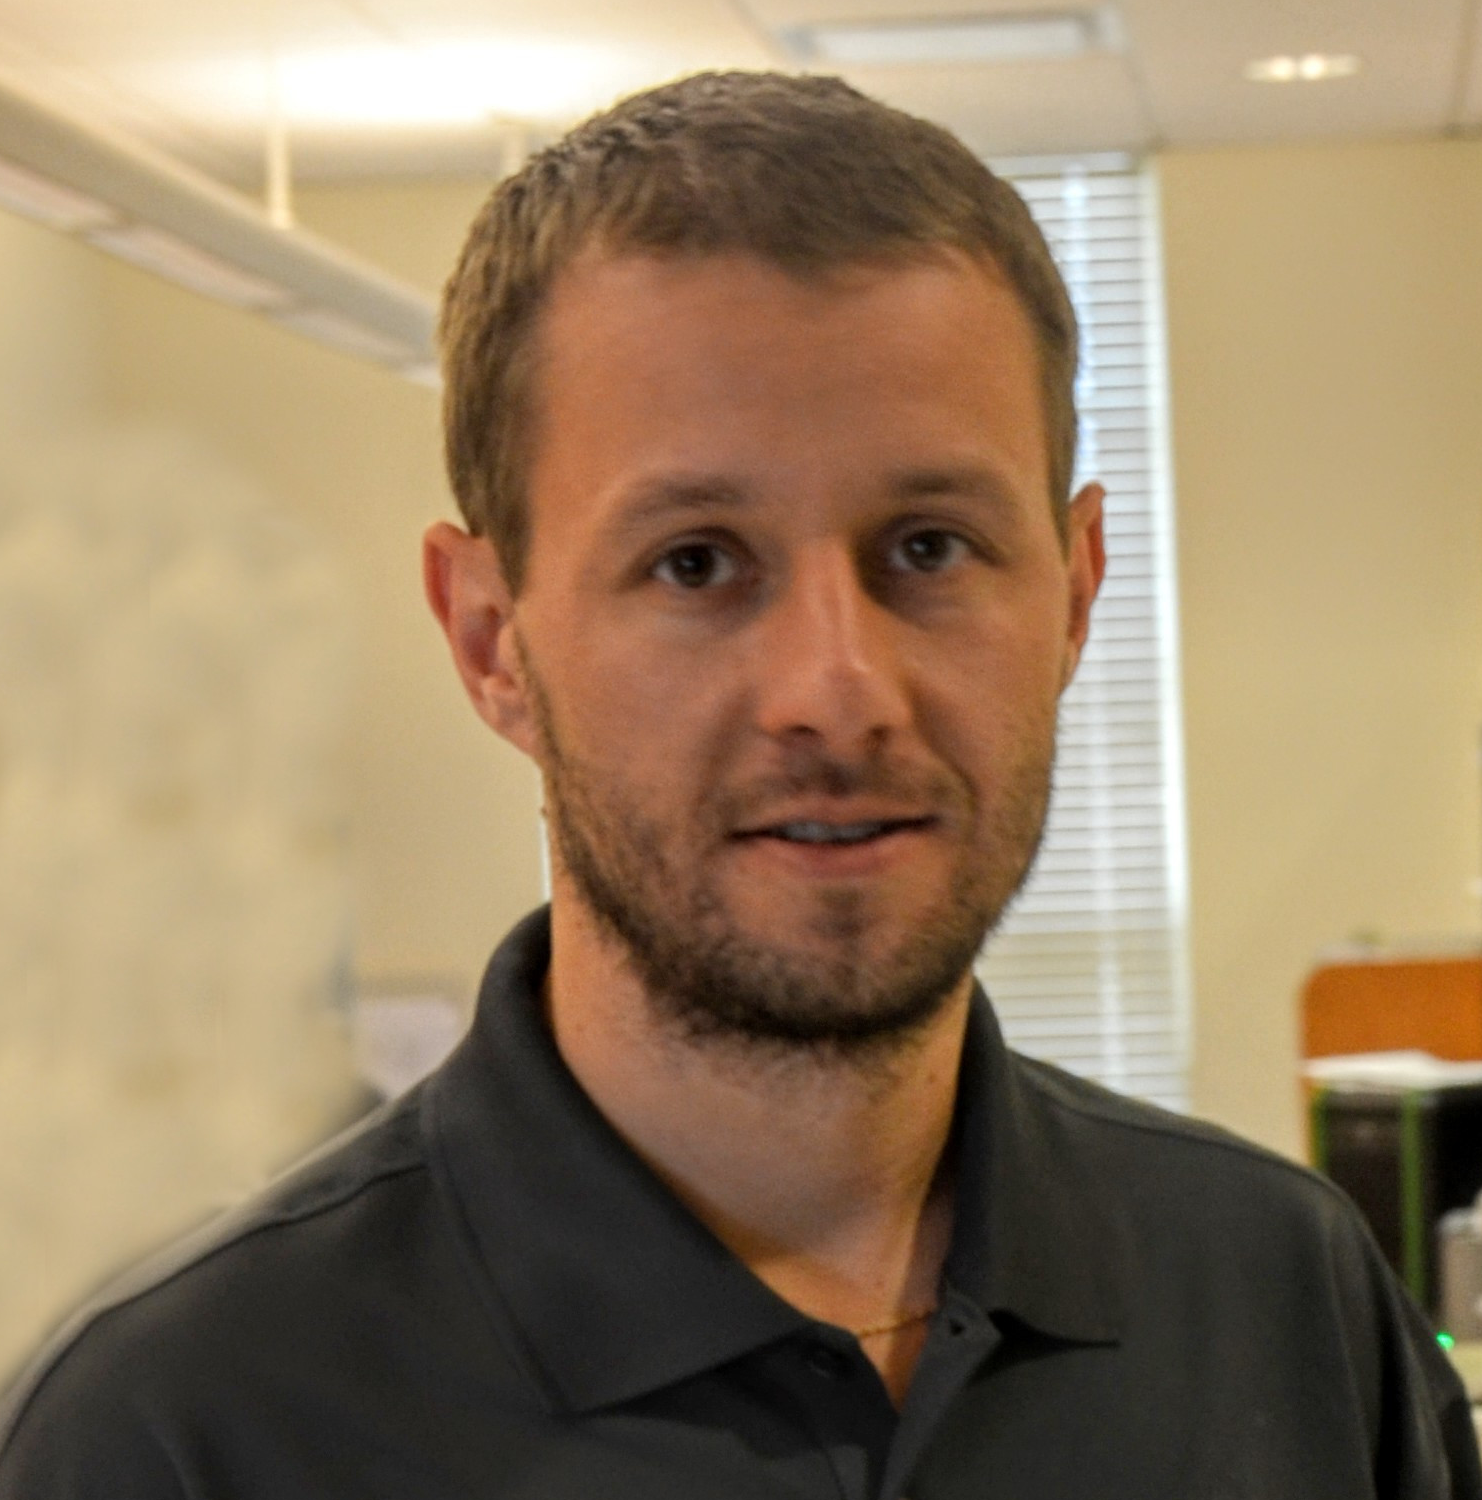
\includegraphics[width=0.5\linewidth]{cristian_cira}\\ \textbf{Cristian Cira}\\ Perfomance Analysis

\column{.3\textwidth}
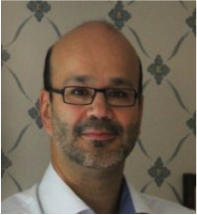
\includegraphics[width=0.5\linewidth]{henric_zazzi}\\ \textbf{Henric Zazzi}\\ Bioinformatics/Genetics
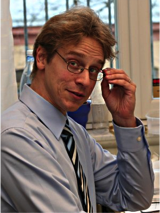
\includegraphics[width=0.5\linewidth]{michael_djurfeldt}\\ \textbf{Michael Djurfeldt}\\ Computational Physics

\column{.3\textwidth}
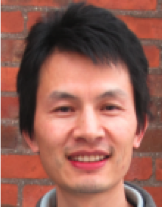
\includegraphics[width=0.5\linewidth]{jing_gong}\\ \textbf{Jing Gong} \\ Scientific Computing
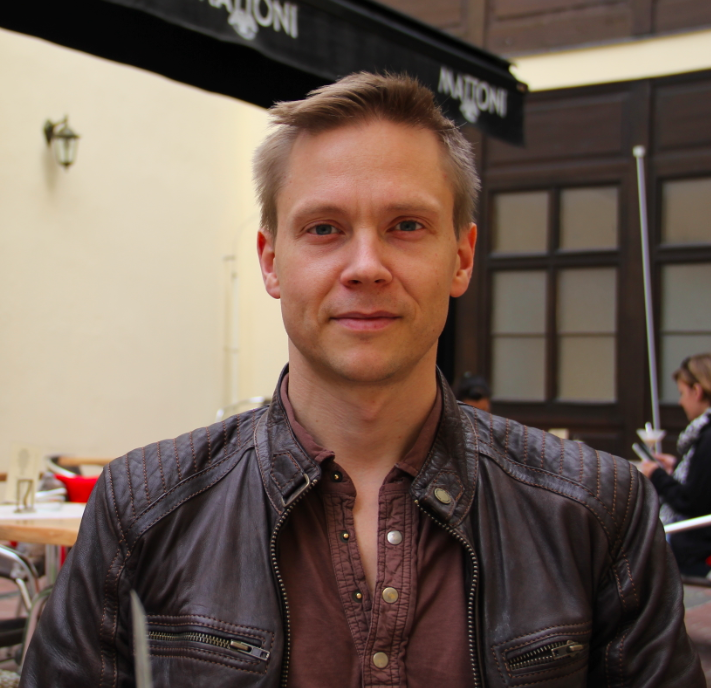
\includegraphics[width=0.5\linewidth]{thor_wikfeldt}\\ \textbf{Thor Wikfeldt} \\ Computational \\ Chemistry

\end{columns}
}}

\subsection*{Services}
\frame{
\frametitle{Services}
\begin{itemize}
\item Access to supercomputers
\item HPC training 
\item Postgraduate degree projects
\item Visualization
\item Support 
\item Expertise in HPC software
\item Access to international HPC facilities
\item Data storage
\end{itemize}
}

\section{Infrastructure}

%\subsection*{Overview}
%\frame{
%\frametitle{What is a cluster?}
%\framesubtitle{\includegraphics[height=0.3\textheight,width=\textwidth]{Titan1}}
%
%\begin{columns}[T]
%\column{.4\textwidth}
%  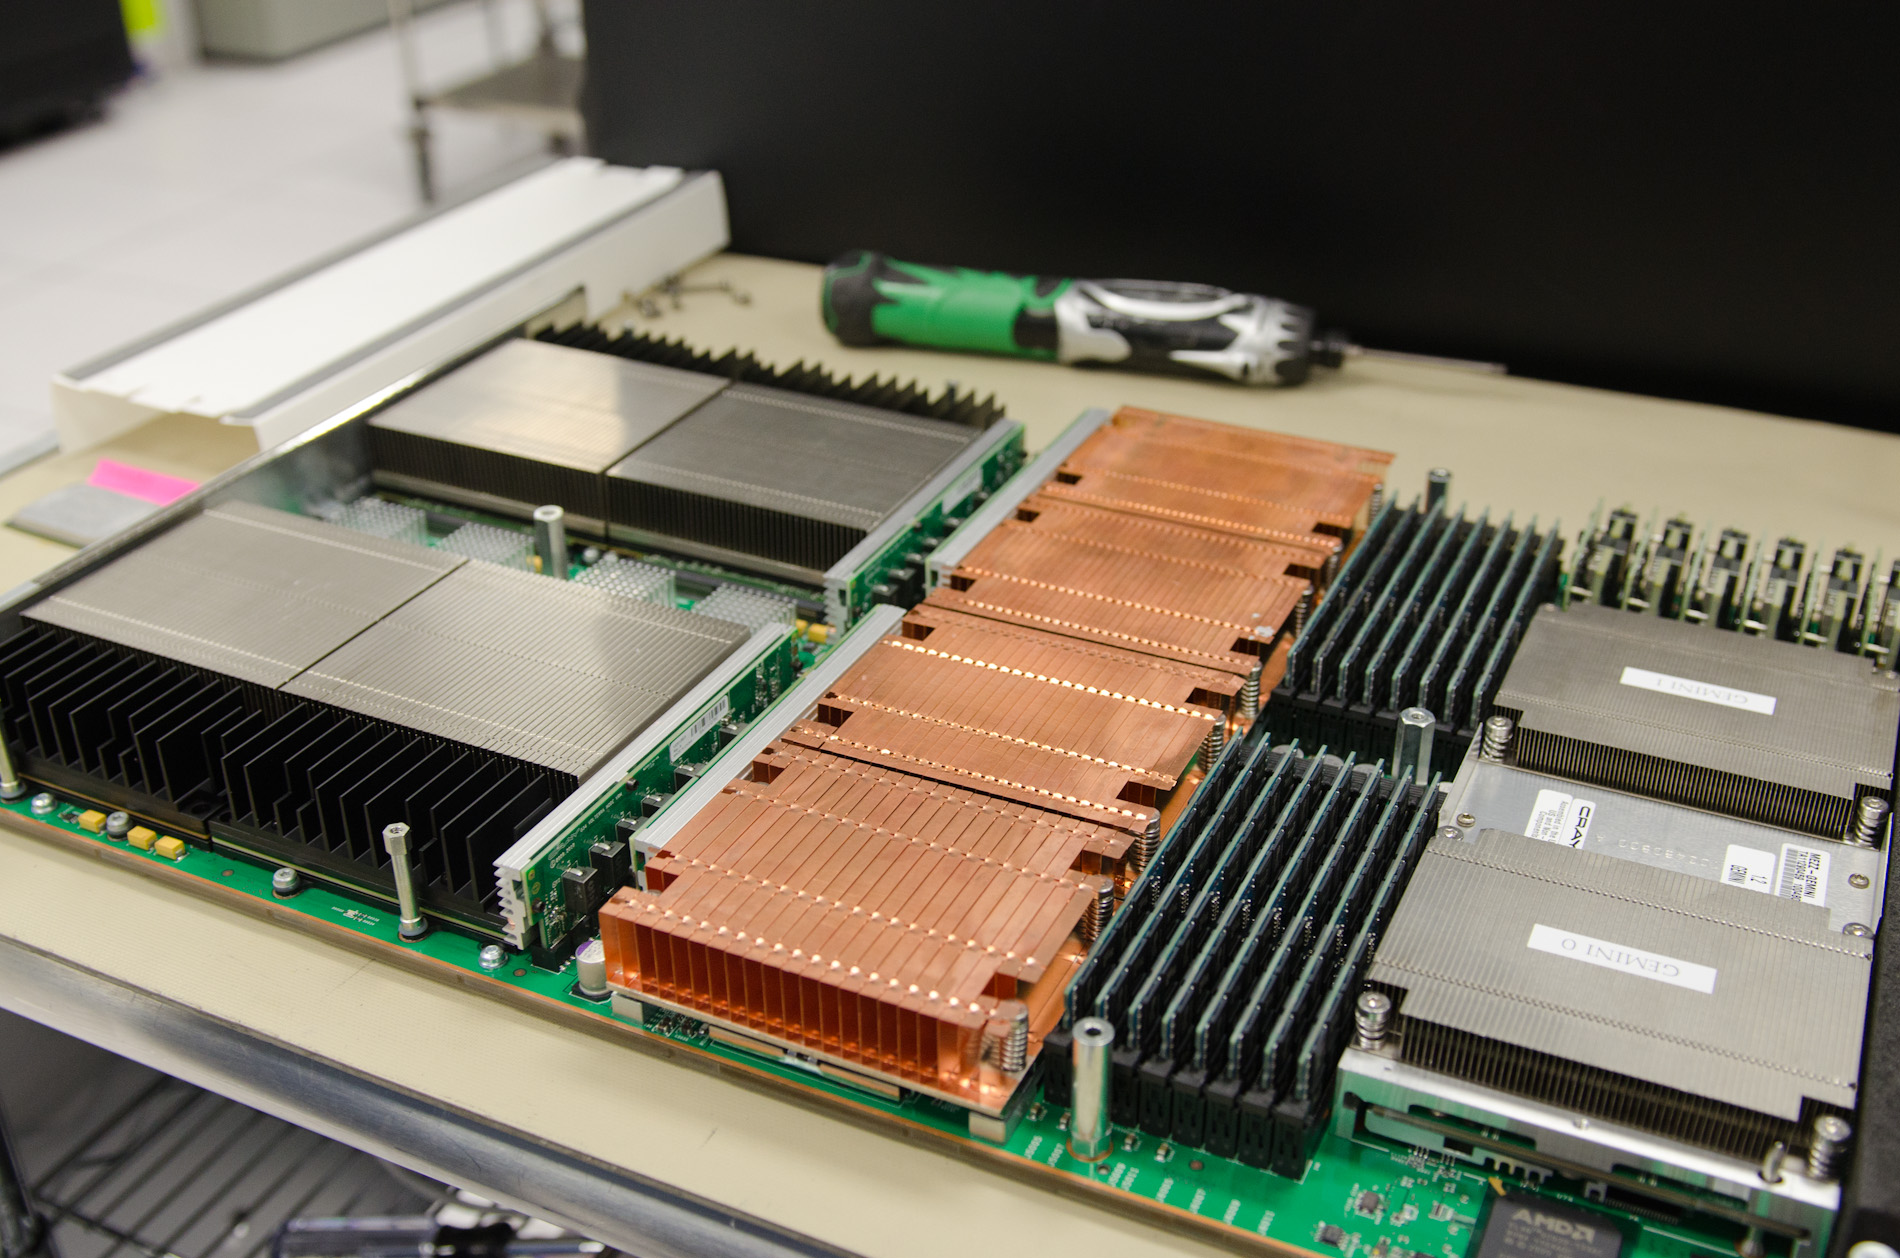
\includegraphics[width=\columnwidth]{TitanIn}
%  \column{.3\textwidth}
%  \begin{itemize}
%    \item Cluster
%    \item Racks
%    \item Blades
%    \item Nodes
%    \item Processors 
%    \item Cores
%  \end{itemize}
%\column{.3\textwidth}
%  \begin{itemize}
%    \item Login nodes
%    \item Compute nodes
%    \item Dedicated nodes
%    \item Transfer nodes
%    \item Service nodes
%  \end{itemize}
%\end{columns}
%}


\subsection{Beskow}
\frame{
\frametitle{Beskow - Cray XC40 system}
\framesubtitle{\hspace{0.2\textwidth}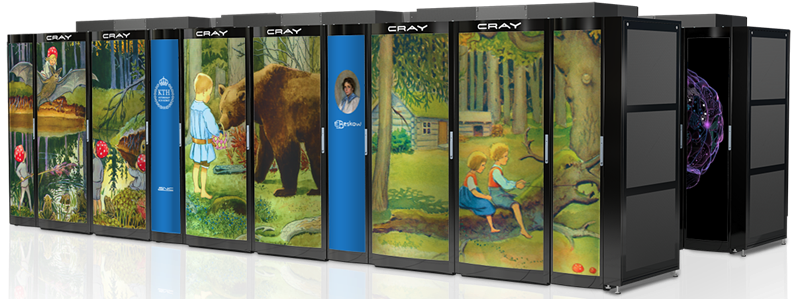
\includegraphics[height=0.3\textheight]{Beskow}}

\begin{alertblock}{}{\alert{Fastest machine in Scandinavia}}\end{alertblock}

\begin{columns}
\column{.6\textwidth}
  \begin{itemize}
    \item Lifetime: Q4 2019
    \item $11$ racks, $2060$ nodes
    \item Intel Haswell processor 2.3 GHz \\ Intel Broadwell processor 2.1 GHz
    \item $67,456$ cores - $32$($36$) cores/node
    \item Aries Dragonfly network topology
    \item $156.4$ TB memory - $64$($128$) GB/node
  \end{itemize}
\column{.4\textwidth}
  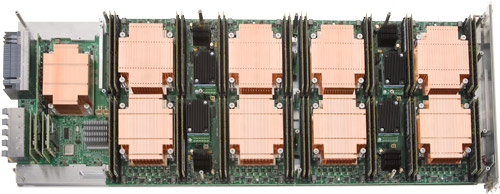
\includegraphics[width=\columnwidth]{xc30-blade}
  \scriptsize\\
  $1$ XC compute blade\\
  $1$ Aries Network Chip ($4$ NICs)\\
  $4$ Dual-socket Xeon nodes\\
  $4$ Memory DIMM / Xeon node
\end{columns}
}

\subsection{Tegner}
\frame{
\frametitle{Tegner}
\framesubtitle{pre/post processing for Beskow}

\begin{columns}
\column{.4\textwidth}
\scriptsize
  \begin{alertblock}{$5$ x $2$TB Fat nodes}
    $4$ x $12$ core Ivy Bridge, $2$TB RAM \\
    $2$ x Nvidia Quadro K420
  \end{alertblock}
  
  \begin{alertblock}{$5$ x $1$TB Fat nodes}
    $4$ x $12$ core Ivy Bridge, $1$TB RAM \\
    $2$ x Nvidia Quadro K420
  \end{alertblock}
  
  \begin{alertblock}{$46$ Thin Nodes}
    $2$ x $12$ core Haswell, $512$GB RAM \\
    Nvidia Quadro K420 GPU
  \end{alertblock}

  \begin{alertblock}{$9$ K80 Nodes}
    $2$ x $12$ core Haswell, $512$GB RAM \\
    Nvidia Tesla K80 GPU
  \end{alertblock}

\column{.6\textwidth}
\normalsize
\centering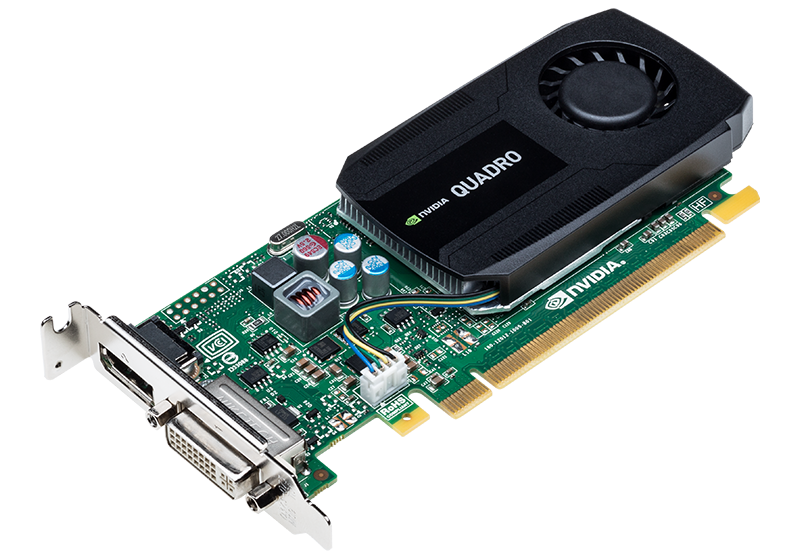
\includegraphics[width=.5\columnwidth]{k420}
  
  \begin{itemize}
    \item Used for pre/post processing data 
    \item Has large RAM nodes
    \item Has nodes with GPUs
    \item Has two transfer nodes
    \item Lifetime: Q4 2019
  \end{itemize}
\end{columns}
}


\subsection*{Summary}
\frame{
\frametitle{Summary of PDC resources}
\framesubtitle{}
\begin{table}
  \begin{tabular}{r|l|l}
   & \alert{Beskow} & \alert{Tegner}\\ \hline \hline
  Cores in each node &  $32/36$ & $48/24$\\\hline
  Nodes &  $1676$ Haswell  & 55 x $24$ Haswell/GPU\\
        &  $384$ Broadwell & 10 x $48$ Ivy bridge\\\hline
  RAM (GB) & $1676$ x $64$GB & $55$ x $512$GB\\
           & $384$ x $128$GB & $5$ x $1$TB\\
           &                 & $5$ x $2$TB\\\hline
  Allocations &&\\
  (core hours per month)&&\\
  Small &	$<5k$&	$<5k$\\
  Medium &	$<200k$&	$<80k$\\
  Large &	$\geq 200k$	 \\\hline
  Availability via SNIC &	yes &	with Beskow\\\hline
  AFS &	login node only &	yes\\
  Lustre &	yes	& yes\\
  \end{tabular}
\end{table}
}

\subsection*{File systems}
\frame{
\frametitle{File Systems}
\begin{block}{Andrew File System (\alert{AFS})}
\begin{itemize}
  \item Distributed file system accessible to any running AFS client
  \item Home directory \\  \url{/afs/pdc.kth.se/home/[initial]/[username]}
  \item Access via Kerberos tickets and AFS tokens
  \item \alert{Not accessible to compute nodes on Beskow}
\end{itemize}
\end{block}

\begin{block}{Lustre File System (\alert{Klemming})}
\begin{itemize}
 \item Open-source massively parallel distributed file system
 \item Very high performance ($5$PB storage - $130$GB/s bandwidth)
 \item NO backup (always move data when done) NO personal quota
 \item Home directory \\  \url{/cfs/klemming/nobackup/[initial]/[username]}
\end{itemize}
\end{block}
}

\frame<presentation:0>[noframenumbering]{
\frametitle{File System Access}
 \begin{tabular}{ccc}
   
  \cellcolor{kthLightGreen} \textbf{AFS} & 
  \cellcolor{kthLightBlue}{Beskow Compute Node} &
  \cellcolor{kthLightBlue}\textbf{CFS}\\
   
  \cellcolor{kthLightGreen} Andrew File System & 
  \cellcolor{kthLightGreen!50!kthLightBlue} Beskow Login Node &  
  \cellcolor{kthLightBlue} Lustre File System\\ 
  
  \cellcolor{kthLightGreen}~ &
  \cellcolor{kthLightGreen!50!kthLightBlue}~ &
  \cellcolor{kthLightBlue}~\\

  \cellcolor{kthLightGreen} & 
  \cellcolor{kthLightGreen!50!kthLightBlue} Tegner Compute Node &  
  \cellcolor{kthLightBlue} \scriptsize{\url {/cfs/klemming/ }\alert{\textbf{nobackup}}\url{/}} \\
  
  
  \cellcolor{kthLightGreen} \scriptsize{\url{/afs/pdc.kth.se/home/}} & 
  \cellcolor{kthLightGreen!50!kthLightBlue} Tegner Login Node &  
  \cellcolor{kthLightBlue} \scriptsize{\url{/[initial]/[username]}} \\

  \cellcolor{kthLightGreen} \scriptsize{\url{/[initial]/[username]}}  &
  \cellcolor{kthLightGreen} &
  \cellcolor{kthLightBlue} \\

  \cellcolor{kthLightGreen} & 
  \cellcolor{kthLightGreen} KTH (Linux) computer &  
  \cellcolor{kthLightBlue} \scriptsize{\url{/cfs/klemming/}\alert{\textbf{scratch}}\url{/}}\\
 
  \cellcolor{kthLightGreen} &
  \cellcolor{kthLightGreen} & 
  \cellcolor{kthLightBlue} \scriptsize{\url{/[initial]/[username]}}\\
   
  \cellcolor{kthLightGreen} & 
  \cellcolor{kthLightGreen} Laptop/Home computer &
  \cellcolor{kthLightBlue}
  \end{tabular}
}

\frame<presentation:0>[noframenumbering]{
\frametitle{File System Access}
 
\begin{tikzpicture}
\begin{scope}[transparency group]
\begin{scope}[blend mode=multiply]
  \coordinate (AFS) at (1,0);
  \coordinate (CFS) at (4,0);
  \coordinate (LARGE) at (9,0);
  %\node at (3,-1) {\alert{\textbf{AFS}}}; 
  \node[align=center,text width=3.1cm] at (2.5,1.5) {\textbf{\alert{Tegner Login Node}}};
  \node[align=center,text width=3.1cm] at (2.5,0) {\textbf{Tegner Compute Node}};
  \node[align=center,opacity=1,text width=1.5cm] at (2.5,-2) {\textbf{Beskow Login Node}};
  
  \node[align=center,text width=2cm] at (6,0) {\textbf{Beskow Compute Node}};
  
  \node[align=left,text width=2.3cm] at (0,2) {\textbf{KTH (Linux) computer}};
  \node[align=center,text width=2.5cm] at (-1,-1) {\textbf{Laptop/Home computer}};
  
  \filldraw[fill=kthLightBlue, draw=black,opacity=0.5,rounded corners=1mm] (AFS) \irregularcircle{3.5cm}{3mm};
  \filldraw[fill=kthLightGreen, draw=black,opacity=0.5,rounded corners=1mm] (CFS) \irregularcircle{3.5cm}{2mm};
\end{scope}
\end{scope}
\end{tikzpicture}

  
}

\section{Accounts}

\subsection*{Access requirements}
\frame{
\frametitle{Access requirements}

\begin{description}
\item [User account] either SUPR or PDC
\item [Time allocation] set the access limits
\end{description}

\begin{alertblock}{Apply for PDC account via SUPR}
\begin{itemize}
  \item http://supr.snic.se
  \item SNIC database of persons, projects, project proposals and more
  \item Apply and link SUPR account to PDC
  \item Valid post address for password
\end{itemize}
\end{alertblock}

\begin{alertblock}{Apply for PDC account via PDC}
\begin{itemize}
  \item http://www.pdc.kth.se/support/accounts/user
  \item Electronic copy of your passport
  \item Valid post address for password 
  \item Membership of specific time allocation 
\end{itemize}
\end{alertblock}

}


\subsection{Time allocations}
\frame{
\frametitle{Time Allocations}
\scriptsize
\begin{block}{\large{Small allocation}}
\begin{itemize}
  \item Applicant can be a PhD student or more senior
  \item Evaluated on a technical level only
  \item Limits is usually $5K$ corehours each month
\end{itemize}
\end{block}

\begin{exampleblock}{\large{Medium allocation}}
\begin{itemize}
  \item Applicant must be a senior scientist in Swedish academia
  \item Evaluated on a technical level only
  \item On large clusters: $200K$ corehours per month
\end{itemize}
\end{exampleblock}

\begin{alertblock}{\large{Large allocation}}
\begin{itemize}
  \item Applicant must be a senior scientist in Swedish academia
  \item Need evidence of successful work at a medium level
  \item Evaluated on a technical and scientific level
  \item Proposal evaluated by SNAC twice a year
\end{itemize}
\end{alertblock}
}

\subsection*{Acknowledgement }
\frame
{
\frametitle{Using resources}

\begin{itemize}
\item All resources are free of charge for Swedish academia
\item Acknowledgement \alert{are} taken into consideration when applying
\item Please acknowledge SNIC/PDC when using these resources:
\end{itemize}
\begin{alertblock}{Acknowledge SNIC/PDC}
The computations/simulations/[SIMILAR] were performed on resources provided by the Swedish National Infrastructure for Computing (SNIC) at [CENTERNAME (CENTER-ACRONYM)]
\end{alertblock}
\begin{alertblock}{Acknowledge people}
NN at [CENTER-ACRONYME] is acknowledged for assistance concerning technical and implementation aspects [OR SIMILAR] in making the code run on the [OR SIMILAR] [CENTER-ACRONYM] resources.
\end{alertblock}
}



\subsection{Authentication}
\begin{frame}[fragile]
\frametitle{Authentication}
\framesubtitle{\alert{\textbf{Kerberos}} Authentication Protocol}
\footnotesize
\begin{exampleblock}{\large{Ticket}}
\begin{itemize}
  \item Proof of users identity
  \item Users use passwords to obtain tickets
  \item Tickets are cached on the user's computer for a specified duration
  \item Tickets \alert{should be created on your local computer}
  \item No passwords are required during the ticket's lifetime
\end{itemize}
\end{exampleblock}

\begin{exampleblock}{\large{Realm}}
Sets boundaries within which an authentication server has authority (\verb|NADA.KTH.SE|)
\end{exampleblock}

\begin{exampleblock}{\large{Principal}}
Refers to the entries in the authentication server database  (\verb|username@NADA.KTH.SE|)
\end{exampleblock}

\end{frame}

\subsection*{Kerberos commands}

\begin{frame}[fragile]
\frametitle{Kerberos commands}

\begin{columns}[t]
\column{.5\textwidth}
\alert{Normal commands:}
\begin{description}
 \item [kinit] generates ticket
 \item [klist] lists kerberos tickets
 \item [kdestroy] destroys ticket file
 \item [kpasswd] changes password
\end{description}

\column{.5\textwidth}
\alert{On KTH-Ubuntu machines:}
\begin{description}
 \item [pdc-kinit] 
 \item [pdc-klist] 
 \item [pdc-kdestroy]
 \item [pdc-kpasswd] 
\end{description}
\end{columns}

\scriptsize
\begin{block}{}
  \begin{verbatim}
    $ kinit --forwardable username@NADA.KTH.SE
    $ klist -Tf
    
    Credentials cache : FILE:/tmp/krb5cc_500
        Principal: username@NADA.KTH.SE
    Issued       Expires     Flags  Principal
    Mar 25 09:45 Mar 25 19:45 FI krbtgt/NADA.KTH.SE@NADA.KTH.SE
    Mar 25 09:45 Mar 25 19:45 FA afs/pdc.kth.se@NADA.KTH.SE
\end{verbatim}
\end{block}
\end{frame}


\begin{frame}[fragile]
\frametitle{Login using Kerberos tickets}

\begin{block}{Get a 7 days forwardable ticket on your local system}
\begin{verbatim}
$ kinit -f -l 7d username@NADA.KTH.SE
\end{verbatim}
\end{block}

\begin{block}{Forward your ticket via ssh and login}
\begin{verbatim}
$ ssh
  -o GSSAPIDelegateCredential=yes
  -o GSSAPIAuthentication=yes
  -o GSSAPIKeyExchange=yes
  username@clustername.pdc.kth.se
\end{verbatim}
\end{block}

\begin{block}{OR, when using \url{~/.ssh/config}}
\begin{verbatim}
$ ssh username@clustername.pdc.kth.se
\end{verbatim}
\end{block}

\alert{Always create a kerberos ticket on your local system}
\alert{https://www.pdc.kth.se/resources/software/login-1}
\end{frame}

\section{Development}
\subsection{Building}
\begin{frame}[fragile]
\frametitle{Compiling, Linking and Running Applications}
\framesubtitle{on HPC clusters}
 \begin{description}
    \item [source code] C / C++ / Fortran ( \verb|.c, .cpp, .f90, .h|  )
    \item [compile] Cray/Intel/GNU compilers
    \item [assemble] into machine code (object files: \verb|.o, .obj| )
    \item [link] Static Libraries (\verb|.lib, .a|  ) \\ Shared Library (\verb|.dll, .so| ) \\ Executables (\verb|.exe, .x| )
    \item ~ 
    \item [request allocation] submit job request to SLURM queuing system \\ \verb|salloc/sbatch|
    \item [run] application on scheduled resources \\ \verb|srun/mpirun|
 \end{description}
\end{frame}

\subsection{Modules}
\begin{frame}[fragile]
\frametitle{Modules}
\framesubtitle{The \textit{modules package} allow for dynamic add/remove of installed software packages to the running environment}

\begin{exampleblock}{Loading modules}
  \begin{verbatim}
  module load 	<software_name>
  module add 	<software_name>
  module use 	<software_name>
  \end{verbatim}
\end{exampleblock}

\begin{exampleblock}{Swapping modules}
  \begin{verbatim}
  module swap 	<software_name_1> <software_name_2>
  \end{verbatim}
\end{exampleblock}

\begin{exampleblock}{Unloading modules}
  \begin{verbatim}
  module unload <software_name>
  \end{verbatim}
\end{exampleblock}
\end{frame}


\begin{frame}[fragile]
\frametitle{Modules }
\framesubtitle{Displaying modules}
\begin{exampleblock}{\$ module list}
\scriptsize
\begin{verbatim}
Currently Loaded Modulefiles:
  1) modules/3.2.6.7
  ...
  20) PrgEnv-cray/5.2.56
\end{verbatim}
\end{exampleblock}

\begin{exampleblock}{\$ module avail [\textit{software\_name}]}
\scriptsize
\begin{verbatim}
-------------------------- /opt/modulefiles -----------------------------
gcc/4.8.1     gcc/4.9.1(default)     gcc/4.9.2     gcc/4.9.3    gcc/5.1.0
\end{verbatim}
\end{exampleblock}

\begin{exampleblock}{\$ module show \textit{software\_name}}
\scriptsize
\begin{verbatim}
------------------------- /opt/modulefiles/gcc/4.9.1 ---------------------
conflict	 gcc 
prepend-path	 PATH /opt/gcc/4.9.1/bin 
prepend-path	 MANPATH /opt/gcc/4.9.1/snos/share/man 
prepend-path	 LD_LIBRARY_PATH /opt/gcc/4.9.1/snos/lib64 
setenv		 GCC_PATH /opt/gcc/4.9.1 
-------------------------------------------------------------------
\end{verbatim}
\end{exampleblock}
\end{frame}

\subsection{Programming environments}
\begin{frame}[fragile]
  \frametitle{Programming Environment Modules}
  \framesubtitle{specific to \alert{Beskow}}

\begin{columns}[t]
\column{.7\textwidth}
  \begin{description}
  \item [Cray] \verb|$ module load PrgEnv-cray|
  \item [Intel] \verb|$ module load PrgEnv-intel|
  \item [GNU] \verb|$ module load PrgEnv-gnu|
  \end{description}
   % \item Module cray-libsci provides BLAS, LAPACK, BLACS, and SCALAPACK
   % \item Module cray-mpich provides MPI
\column{.3\textwidth}
    \begin{verbatim}
$ cc	source.c
$ CC	source.cpp
$ ftn	source.F90
  \end{verbatim}
\end{columns}
  \begin{exampleblock}{Compiler wrappers : \alert{\textbf{cc} \textbf{CC} \textbf{ftn}}}
    \alert{Advantages}\\
    Compiler wrappers will automatically 
    \begin{itemize}
      \item link to BLAS, LAPACK, BLACS, SCALAPACK, FFTW\\
      \item use MPI wrappers\\
    \end{itemize}
    \alert{Disadvantage}\\
    Sometimes you need to edit Makefiles which are not designed for Cray 
\end{exampleblock}
\end{frame}


\subsection{Compilers}
\begin{frame}[fragile]
\frametitle{Compiling serial and/or parallel code}
\framesubtitle{specific to \alert{Tegner}}

\begin{columns}[t]
\column{.45\textwidth}
\begin{exampleblock}{GNU Compiler Collection (\textbf{gcc})}
  \scriptsize
  \begin{verbatim}
$ module load 	gcc openmpi
$ gcc	   -fopenmp source.c
$ g++	   -fopenmp source.cpp
$ gfortran -fopenmp source.F90
$ mpicc	   -fopenmp source.c
$ mpicxx   -fopenmp source.cpp
$ mpif90   -fopenmp source.F90
  \end{verbatim}
  \end{exampleblock}

  \begin{exampleblock}{Portland Group Compilers (\textbf{pgi}) }
  \scriptsize
  \begin{verbatim}
$ module load 	pgi
$ pgcc  -mp source.c
$ pgcpp -mp source.cpp
$ pgf90 -mp source.F90
  \end{verbatim}
  \end{exampleblock}

\column{.45\textwidth}

  \begin{exampleblock}{Intel compilers (\textbf{i-compilers})}
  \scriptsize
  \begin{verbatim}
  $ module load i-compilers
  $ icc   -openmp source.c	
  $ icpc  -openmp source.cpp
  $ ifort -openmp source.F90
  $ module load i-compilers intelmpi
  $ mpiicc 	-openmp source.c
  $ mpiicpc 	-openmp source.cpp
  $ mpiifort 	-openmp source.F90
  \end{verbatim}
  \end{exampleblock}

  \begin{exampleblock}{CUDA compilers (\textbf{cuda})}
  \scriptsize
  \begin{verbatim}
  $ module load cuda
  $ nvcc source.cu
  $ nvcc -arch=sm_37  source.cu
  \end{verbatim}
  \end{exampleblock}

\end{columns}
\end{frame}



\section{Running jobs}
\frame{
\frametitle{How to run programs}
\begin{itemize}
  \item After login we are on a \textit{login node} used only for:
  \begin{itemize}
    \item submitting jobs,
    \item editing files,
    \item compiling small programs,
    \item other computationally light tasks.
  \end{itemize}
  \item \alert{Never run calculations interactively on the login node} 
  \item Instead, request compute resources \textit{interactively} or via \textit{batch script} \\~

  \item All jobs must be connected to a time allocation
  \item For courses, PDC sets up a \textit{reservation} for resources \\~

  \item To manage the workload on the clusters, PDC uses a queueing/batch system

  \end{itemize}
 }


\subsection{SLURM}
\frame{
\frametitle{SLURM workload manager}
\framesubtitle{Simple Linux Utility for Resource Management}

\begin{itemize}
 \item Open source, fault-tolerant, and highly scalable cluster management and job scheduling system
 \begin{itemize}
  \item \alert{Allocates} exclusive and/or non-exclusive access to \alert{resources} for some duration of time
  \item Provides a framework for \alert{starting}, \alert{executing}, and \alert{monitoring} work on the set of allocated nodes
  \item \alert{Arbitrates contention} for resources by managing a queue 
 \end{itemize}
 \item Job Priority computed based on 
 \begin{description}
    \item [Age] the length of time a job has been waiting
    \item [Fair-share] the difference between the portion of the computing resource that has been promised and the amount of resources that has been consumed
    \item [Job size] the number of nodes or CPUs a job is allocated
    \item [Partition] a factor associated with each node partition
%    \item [QOS] a factor associated with each Quality Of Service
 \end{description}
\end{itemize}
}

\subsection*{SLURM commands}

\begin{frame}[fragile]
\frametitle{Interactive session \hfill \alert{\textbf{salloc}}}

\begin{exampleblock}{Request an interactive allocation of resources}
  \begin{verbatim}
  $ salloc -A <account> -t <d-hh:mm:ss> -N <nodes>
  salloc: Granted job allocation 123456
  \end{verbatim}
\end{exampleblock}

\begin{exampleblock}{Run application on \alert{\textbf{Beskow}}}
  \begin{verbatim}
  $ srun -n <PEs> ./binary.x
  #PEs 	- number of processing elements (MPI processes)
  \end{verbatim}
\end{exampleblock}
  
  
\begin{exampleblock}{Run application on \alert{\textbf{Tegner}}}

  \begin{verbatim}
  $ mpirun -np <cores> ./binary.x
  \end{verbatim}
\end{exampleblock}
\end{frame}

\begin{frame}[fragile]
\frametitle{Launch batch jobs \hfill  \alert{\textbf{sbatch}}}
\begin{exampleblock}{Submit the job to SLURM queue}
  \begin{verbatim}
$ sbatch <script>
Submitted batch job 958287
  \end{verbatim}
\end{exampleblock}

\scriptsize
The script should contain all necessary data to identify the account and requested resources 
\begin{exampleblock}{Example of request to run myexe for 1 hour on 4 nodes}
  \begin{verbatim}
#!/bin/bash -l

#SBATCH -A summer-2019
#SBATCH -J myjob
#SBATCH -t 1:00:00
#SBATCH --nodes=4
#SBATCH --ntasks-per-node=32
#SBATCH -e error_file.e
#SBATCH -o output_file.o

srun -n 128 ./myexe > my_output_file
  \end{verbatim}
\end{exampleblock}

\end{frame}

\begin{frame}[fragile]
\frametitle{Monitoring and/or cancelling running jobs }
\begin{alertblock}{\textbf{squeue} -u  \$USER}
  Displays all queue and/or running jobs that belong to the user
\tiny
  \begin{verbatim}
cira@beskow-login2:~> squeue -u cira
 JOBID     USER ACCOUNT           NAME  ST REASON    START_TIME                TIME  TIME_LEFT NODES  CPUS
957519   cira pdc.staff      VASP-test   R None      2016-08-15T08:15:24    6:09:42   17:49:18    16  1024
957757   cira pdc.staff      VASP-run    R None      2016-08-15T11:14:20    3:10:46   20:48:14    128 8192
  \end{verbatim}
\end{alertblock}

\begin{alertblock}{\textbf{scancel} [job]}
Stops a running job or removes a pending one from the queue
\tiny
  \begin{verbatim}
cira@beskow-login2:~> scancel 957519
salloc: Job allocation 957891 has been revoked.

cira@beskow-login2:~> squeue -u cira
JOBID     USER ACCOUNT           NAME  ST REASON    START_TIME                TIME  TIME_LEFT NODES  CPUS
957757   cira pdc.staff      VASP-run    R None      2016-08-15T11:14:20    3:10:46   20:48:14    128 8192
  \end{verbatim}
\end{alertblock}
\end{frame}

%\fontsize{12pt}{13.2}\selectfont
\section{How to get help}

\frame{
\frametitle{How to start your project}
\begin{itemize}
\item Proposal for a small allocation
\item Develop and test your code
\item Run and evaluate scaling
\item Proposal for a medium (large) allocation
\end{itemize}
}

\subsection*{PDC suppport}
\frame{
\frametitle{PDC support}
\begin{itemize}
  
  \item Many questions can be answered by reading the web documentation: \alert{\url{https://www.pdc.kth.se/support}}
  \item Preferably contact PDC support by email: \alert{\url{support@pdc.kth.se}}
  \begin{itemize}
    \item you get a ticket number.
    \item always include the ticket number in follow-ups/replies\\ they look like this: [SNIC support \#12345]
  \end{itemize}
  \item Or by phone: \alert{$+46$ $(0)8$ $790$ $7800$}
  \item You can also make an appointment to \alert{come and visit}.
\end{itemize}
}


\subsection*{How to report problems}
\frame{
\frametitle{How to report problems \hfill  \alert{\url{support@pdc.kth.se}}}
\begin{itemize}
  \item Do not report new problems by replying to old/unrelated tickets.
  \item Split unrelated problems into separate email requests.
  \item Use a descriptive subject in your email.
  \item Give your PDC user name.
  \item Be as specific as possible.
  \item For problems with scripts/jobs, give an example.\\ Either send the example or make it accessible to PDC support.
  \item Make the problem example as small/short as possible.
  \item Provide all necessary information to reproduce the problem.
  \item If you want the PDC support to inspect some files, make sure that the files are readable.
  \item Do not assume that PDC support personnel have admin rights\\ to see all your files or change permissions.
\end{itemize}
}

\frame{\huge\centering Questions...?}
\section*{Login and running}

\begin{frame}[fragile]
  \frametitle{Hands-on exercise}

\footnotesize
\begin{exampleblock}{\large{Login}}
\begin{itemize}
  \item Some configuration steps are needed to log in to PDC 
  \item Depends on OS: https://www.pdc.kth.se/support/documents/login/login.html
  \item In short, Kerberos and SSH supporting GSSAPI key exchange must be installed 
  \item If needed, you will receive help to connect from your own laptops
\end{itemize}
\end{exampleblock}

\begin{exampleblock}{\large{Exercises}}
\begin{itemize}
  \item You will now practice key steps in using PDC resources
  \item The example source code and batch scripts can be found at \verb|/afs/pdc.kth.se/home/k/kthw/Public/pdc_test.tar.gz|,
    or in the GitHub repository \verb|https://github.com/PDC-support/introduction-to-pdc| (in the intro-course branch)
\end{itemize}
\end{exampleblock}

\end{frame}


%-------------------------------------------------------------------------------------
\begin{frame}[fragile]
  \frametitle{Login}
\begin{itemize}
  \item Start by logging in to Beskow
  \item Where are you after login?
    \begin{itemize}
      \item What is your current directory?
      \item What's the name of the login node?
    \end{itemize}
  \item Have a look at the currently running processes on the login node
\end{itemize}
\end{frame}


%-------------------------------------------------------------------------------------
\begin{frame}[fragile]
  \frametitle{Login}
\begin{exampleblock}{{Answer}}
    \verbatimfont{\footnotesize}
    \begin{itemize}
    \item The \verb|pwd| command shows your current directory:
    \begin{verbatim}
      $ pwd
      /afs/pdc.kth.se/home/k/kthw
    \end{verbatim}

    \item The \verb|hostname| command shows the hostname of the login node:
    \begin{verbatim}
      $ hostname
      beskow-login2.pdc.kth.se
    \end{verbatim}

    \item The \verb|top| command shows a snapshot of currently running processes:
    \begin{verbatim}
      $ top
    \end{verbatim}

    \item Note that the login node is a shared resource!
    \end{itemize}

\end{exampleblock}
\end{frame}


%-------------------------------------------------------------------------------------
\begin{frame}[fragile]
  \frametitle{Disk quota, listing projects (allocations)}
\begin{itemize}
  \item Check your AFS disk quota (hint: you will need the \verb|fs| command, type \verb|fs help| to see available subcommands)
  \item Go to your klemming nobackup directory. Can you run \verb|fs| there?
  \item Check which allocation(s) you belong to using the \verb|projinfo| command
    \begin{itemize}
      \item Check all options of \verb|projinfo| using the \verb|-h| flag
      \item How much have your allocations been used, and for how long are they valid?
    \end{itemize}
\end{itemize}
\end{frame}


%-------------------------------------------------------------------------------------
\begin{frame}[fragile]
  \frametitle{Disk quota, listing projects (allocations)}
\begin{exampleblock}{{Answer}}
    \verbatimfont{\footnotesize}
    \begin{itemize}
    \item The \verb|fs lq| command shows the name of the AFS volume of your home directory, your disk quota and usage:
    \begin{verbatim}
      $ fs lq
    \end{verbatim}

    \item \verb|fs lq| only works on AFS. You can type \verb|df -h .| instead, but there's no quota on your klemming usage:
    \begin{verbatim}
      $ df -h .
Filesystem     Size  Used Avail Use% Mounted on
...:/klemming  5.2P  4.4P  730T  86% /cfs/klemming
    \end{verbatim}

    \item The \verb|projinfo| command accesses a database that contains logs of all allocations 
    \begin{verbatim}
      $ projinfo
    \end{verbatim}

    \end{itemize}

\end{exampleblock}
\end{frame}




%-------------------------------------------------------------------------------------
\begin{frame}[fragile]
  \frametitle{Working with modules}
\begin{itemize}
  \item List the modules that are currently loaded (hint: type \verb|module help|)
  \item List all the modules that are available on Beskow
  \item List all available modules named \verb|PrgEnv|
  \item Swap from the \verb|PrgEnv-cray| to the \verb|PrgEnv-gnu| module
\end{itemize}
\end{frame}


%-------------------------------------------------------------------------------------
\begin{frame}[fragile]
  \frametitle{Working with  modules}
\begin{exampleblock}{{Answer}}
    \verbatimfont{\footnotesize}
    \begin{itemize}
    \item Listing all loaded modules and all available modules is done like this:
    \begin{verbatim}
      $ module list
      $ module avail
    \end{verbatim}

    \item To list all modules matching a pattern (like PrgEnv), type
    \begin{verbatim}
      $ module avail PrgEnv
    \end{verbatim}

    \item To swap programming environments (i.e. compiler environments), type
    \begin{verbatim}
      $ module swap PrgEnv-cray PrgEnv-gnu
    \end{verbatim}
    After swapping these modules, the compiler wrappers \verb|CC, cc| and \verb|ftn| point to the GNU compilers (instead of the 
    Cray compilers)

    \end{itemize}

\end{exampleblock}
\end{frame}

%-------------------------------------------------------------------------------------
\begin{frame}[fragile]
  \frametitle{Compiling code}
\begin{itemize}
  \item Copy the tarball \verb|/afs/pdc.kth.se/home/k/kthw/Public/pdc_test.tar.gz| to  
    your nobackup directory, and unpack it
  \item Now compile the MPI example code \verb|hello_world_mpi.c|
    \begin{itemize}
      \item Do you need to load any MPI libraries?
      \item What compiler will be used when using the \verb|cc| compiler wrapper?
    \end{itemize}
\end{itemize}
\end{frame}


%-------------------------------------------------------------------------------------
\begin{frame}[fragile]
  \frametitle{Compiling code}
\begin{exampleblock}{{Answer}}
    \verbatimfont{\footnotesize}
    \begin{itemize}
    \item Copying and extracting the tarball to your klemming directory:
    \begin{verbatim}
      $ cd /cfs/klemming/nobackup/k/kthw
      $ cp /afs/pdc.kth.se/home/k/kthw/Public/pdc_test.tar.gz .
      $ tar zxf pdc_test.tar.gz
      $ cd pdc_test
    \end{verbatim}

    \item When using the compiler wrappers CC, cc and ftn, no MPI or numerical libraries need to be loaded 
      or linked to explicitly!
    \begin{verbatim}
      $ cc -o hello_world_mpi hello_world_mpi.c
    \end{verbatim}
    \item Which compiler did we just compile with?
    \begin{verbatim}
      $ cc --version
      gcc (GCC) 4.9.1 20140716 (Cray Inc.)
    \end{verbatim}

    \end{itemize}

\end{exampleblock}
\end{frame}


%-------------------------------------------------------------------------------------
\begin{frame}[fragile]
  \frametitle{Submitting jobs}
\begin{itemize}
  \item Open the batch script \verb|sbatch_beskow.sh| in your favorite editor (emacs or vim)
    \begin{itemize}
      \item Set the allocation ID to \verb|edu18.intropdc|
      \item Set that the job should run on two nodes, with 16 processes running on each node
      \item Set the requested time of the job to 2 minutes
    \end{itemize}
  \item Submit the job to the SLURM queue!
  \item Monitor the queue to see if your job is running
  \item What output did you get?
\end{itemize}
\end{frame}


%-------------------------------------------------------------------------------------
\begin{frame}[fragile]
  \frametitle{Submitting jobs}
\begin{exampleblock}{{Answer}}
    \verbatimfont{\footnotesize}
    \begin{itemize}
    \item The allocation, number of nodes and time are set with these flags
    \begin{verbatim}
      #SBATCH -A edu18.intropdc
      #SBATCH -t 0:02:00
      #SBATCH --nodes=2
    \end{verbatim}

    \item If you want to run 32 MPI processes in total, with 16 processes on each node, both the \verb|-n| and \verb|-N| flags 
      to \verb|aprun| must be used:
    \begin{verbatim}
      aprun -n 32 -N 16 ./hello_world_mpi
    \end{verbatim}

    \item The job is submitted and monitored like this:
    \begin{verbatim}
      $ sbatch sbatch_beskow.sh
      $ squeue -u <username>
    \end{verbatim}

    \item The output gets written to a default filename:
    \begin{verbatim}
      $ cat slurm-2559495.out
      Hello world from rank 0 out of 32 process
      Hello world from rank 4 out of 32 process
      ...
    \end{verbatim}

    \end{itemize}

\end{exampleblock}
\end{frame}


%-------------------------------------------------------------------------------------

\begin{frame}[fragile]
  \frametitle{SSH}
  \begin{alertblock}{SSH configuration (Linux and Mac)}
    \verbatimfont{\footnotesize}
    \begin{verbatim}
kthw@local~$ cat .ssh/config
# Hosts we want to authenticate to with Kerberos
Host *.kth.se *.kth.se.
# User authentication based on GSSAPI is allowed
GSSAPIAuthentication yes
# Key exchange based on GSSAPI may be used for server authentication
GSSAPIKeyExchange yes
# Hosts to which we want to delegate credentials
Host *.csc.kth.se *.csc.kth.se. *.nada.kth.se *.nada.kth.se. \
     *.pdc.kth.se *.pdc.kth.se.
# Forward (delegate) credentials (tickets) to the server.
GSSAPIDelegateCredentials yes
# Prefer GSSAPI key exchange
PreferredAuthentications gssapi-keyex,gssapi-with-mic
# All other hosts
Host *

 \end{verbatim}
\end{alertblock}

\end{frame}

%-------------------------------------------------------------------------------------

\begin{frame}[fragile]
  \frametitle{Kerberos}
  \begin{alertblock}{Kerberos configuration (Linux and Mac)}
    \verbatimfont{\footnotesize}
    \begin{verbatim}

kthw@local~$ cat /etc/krb5.conf
[domain_realm]
   .pdc.kth.se = NADA.KTH.SE
[appdefaults]
   forwardable = yes
   forward = yes
   krb4_get_tickets = no
[libdefaults]
   default_realm = NADA.KTH.SE
   dns_lookup_realm = true
   dns_lookup_kdc = true

 \end{verbatim}
\end{alertblock}

\end{frame}


%-------------------------------------------------------------------------------------

\begin{frame}[fragile]
  \frametitle{Kerberos}
  \begin{alertblock}{Create and list tickets}
    \verbatimfont{\footnotesize}
    \begin{verbatim}
kthw@local~$ klist
klist: No credentials cache found
      
kthw@local~$ kinit -f kthw@NADA.KTH.SE
Password for kthw@NADA.KTH.SE:

kthw@local~$ klist -Tf  
Ticket cache: KCM:501
Default principal: kthw@NADA.KTH.SE

Valid starting       Expires              Service principal
08/03/2017 16:39:56  08/04/2017 16:39:50  krbtgt/NADA.KTH.SE@NADA.KTH.SE
   Flags: FIA

  \end{verbatim}
  \end{alertblock}

\end{frame}


%-------------------------------------------------------------------------------------


\begin{frame}[fragile]
  \frametitle{Login}
  \begin{alertblock}{Log in to Beskow, check ticket}
    \verbatimfont{\footnotesize}
    \begin{verbatim}

kthw@local:~$ ssh kthw@beskow.pdc.kth.se
kthw@beskow-login2:~$ klist -f

Credentials cache: FILE:/tmp/krb5cc_H26527
    Principal: kthw@NADA.KTH.SE

Issued                Expires             Flags    Principal
Aug  3 16:41:51 2017  Aug  4 16:39:50 2017  FfA    krbtgt/NADA.KTH.SE@NADA.KTH.SE
Aug  3 16:41:52 2017  Aug  4 16:39:50 2017  fA     afs/pdc.kth.se@NADA.KTH.SE
Aug  3 16:41:52 2017  Aug  4 16:39:50 2017  fA     afs@NADA.KTH.SE

 \end{verbatim}
\end{alertblock}



\end{frame}


%-------------------------------------------------------------------------------------


\begin{frame}[fragile]
  \frametitle{Modules}
  \begin{alertblock}{Inspect module system}
    \verbatimfont{\footnotesize}
    \begin{verbatim}

kthw@beskow-login2:~$ module list
...
kthw@beskow-login2:~$ module avail
...
kthw@beskow-login2:~$ module avail gcc
...
kthw@beskow-login2:~$ CC -V
Cray C++ : Version 8.3.4  Mon Aug 07, 2017  15:04:06
kthw@beskow-login2:~$ module swap PrgEnv-cray PrgEnv-gnu
kthw@beskow-login2:~$ CC --version
g++ (GCC) 4.9.1 20140716 (Cray Inc.)

 \end{verbatim}
\end{alertblock}



\end{frame}


%-------------------------------------------------------------------------------------

\begin{frame}[fragile]
  \frametitle{Interactive job on Beskow}
  \begin{alertblock}{Go to Klemming and start interactive session}
    \verbatimfont{\footnotesize}
    \begin{verbatim}

kthw@beskow-login2:~$ cd /cfs/klemming/nobackup/k/kthw/

# (command line shortened below here)
$ salloc -A edu17.intrompi -N 1 -t 0:10:0 --res=edu-Dec-11
salloc: Granted job allocation 1733496

$ hostname
beskow-login2.pdc.kth.se

$ aprun -n 1 hostname
nid01610

$ exit
salloc: Relinquishing job allocation 1733497
salloc: Job allocation 1733497 has been revoked.

 \end{verbatim}
\end{alertblock}



\end{frame}


%-------------------------------------------------------------------------------------

\begin{frame}[fragile]
  \frametitle{Interactive job on Beskow}
  \begin{alertblock}{We compile and run MPI and OpenMP codes}
    \verbatimfont{\footnotesize}
    \begin{verbatim}

kthw@beskow-login2:~$ mkdir -p /cfs/klemming/nobackup/k/kthw/mpi_course
kthw@beskow-login2:~$ cd /cfs/klemming/nobackup/k/kthw/mpi_course
$ cp ~kthw/Public/intro_mpi_dec2017/hello_world.f90 .
$ module swap PrgEnv-cray PrgEnv-gnu
$ salloc -A edu17.intrompi --res=edu-Dec-11 -N 1 -t 0:10:0
salloc: Granted job allocation 1733496
$ ftn -O2 hello_world.f90 -o hello.x
$ aprun -n 32 ./hello.x

$ cp ~kthw/Public/intro_mpi_dec2017/omp_hello.c .
$ cc -fopenmp omp_hello.c -o omp_hello.x
$ export OMP_NUM_THREADS=32
$ aprun -n 1 -d 32 ./omp_hello.x

 \end{verbatim}
\end{alertblock}



\end{frame}


%-------------------------------------------------------------------------------------


\begin{frame}[fragile]
  \frametitle{Batch job}
  \begin{alertblock}{Compile code and write batch script (Beskow)}
    \verbatimfont{\footnotesize}
    \begin{verbatim}

$ cp ~/Public/intro_mpi_dec2017/hello_world.f90 .
$ ftn -o hello_world.x hello_world.f90

$ cat <<EOF > submit.bash
#!/bin/bash -l

#SBATCH -A edu17.intrompi
#SBATCH --reservation=edu-Dec-11
#SBATCH -J myjob
#SBATCH -t 0:10:00
#SBATCH -N 1
#SBATCH -e error_file.e
#SBATCH -o output_file.o

aprun -n 32 ./hello_world.x > my_output_file 2>&1

EOF

 \end{verbatim}
\end{alertblock}


\end{frame}


%-------------------------------------------------------------------------------------

\begin{frame}[fragile]
  \frametitle{Batch job}
  \begin{alertblock}{Submit and monitor job}
    \verbatimfont{\footnotesize}
    \begin{verbatim}

$ sbatch submit.bash
$ squeue -u kthw
JOBID USER ACCOUNT NAME  ST REASON START_TIME TIME TIME_LEFT NODES CPUS
1735211 kthw pdc.sta myjob R None 2017-08-07T16:31:01 0:00 10:00 1 64

$ cat my_output_file
 Hello from rank           31  of           32
 Hello from rank           13  of           32
 Hello from rank           26  of           32
 Hello from rank           10  of           32
 Hello from rank           17  of           32
 Hello from rank           14  of           32
 Hello from rank            1  of           32
...


 \end{verbatim}
\end{alertblock}


\end{frame}


%-------------------------------------------------------------------------------------


\frame{\huge\centering Questions...?}


\end{document}


